%%%%%%%%%%%%%%%%%%%%%%%%%%%%%%%%%%%%%%%%%%%
%                                         %
% Title   : m_d.tex                       %
% Subject : Maintenance manual of Scotch  %
%           Data structure explanations   %
% Author  : Francois Pellegrini           %
%                                         %
%%%%%%%%%%%%%%%%%%%%%%%%%%%%%%%%%%%%%%%%%%%

\section{Data structure explanations}
\label{sec-data}

This section explains some of the data structures implemented in
\scotch\ and \ptscotch.

\subsection{\texttt{Graph}}
\label{sec-data-graph}

Graphs are the fundamental underlying data structures of all the
algorithms implemented in \scotch. The \texttt{Graph} structure is the
foundational data structure, from which subclasses will be derived,
according to the specific needs of the \scotch\ modules. It is
sometimes referred to as the \textit{source graph} structure, with
respect to the \textit{target architecture} \texttt{Arch} onto which
source graphs are to be mapped.

The \texttt{Graph} structure, being a foundational data structure,
does not possess any variable fields related to actual computations,
\eg, partition state variables or an execution context. Such fields
will be found in \textit{active} graphs, \eg, \texttt{Bgraph},
\texttt{Kgraph}, \texttt{Vgraph}.

A \texttt{Graph} is described by means of adjacency lists. These data
are stored in arrays and scalars of type \texttt{SCOTCH\_Num}, as
shown in Figures~\ref{fig-lib-graf-one}
and~\ref{fig-lib-graf-two}. The \texttt{Graph} fields have the
following meaning:
\begin{itemize}
\iteme[\texttt{baseval}]
Base value for all array indexing.
\iteme[\texttt{vertnbr}]
Number of vertices in graph.
\iteme[\texttt{edgenbr}]
Number of arcs in graph. Since edges are represented by both of their
ends, the number of edge data in the graph is twice the number of
graph edges.
\iteme[\texttt{verttax}]
Based array of start indices in $\mathtt{edgetax}$ of vertex
adjacency sub-arrays.
\iteme[\texttt{vendtax}]
Based array of after-last indices in $\mathtt{edgetax}$ of vertex
adjacency sub-arrays.
For any vertex $i$, with $\mathtt{baseval} \leq i < (\mathtt{vertnbr}
+ \mathtt{baseval})$, $(\mathtt{vendtax[}i\mathtt{]}
-\mathtt{verttax[}i\mathtt{]})$ is the degree of vertex $i$, and the
indices of the neighbors of $i$ are stored in $\mathtt{edgetax}$ from
$\mathtt{edgetax[\lbt verttax[}i\mathtt{]]}$ to $\mathtt{edgetax[\lbt
vendtax[}i\mathtt{]} - 1\mathtt{]}$, inclusive.

When all vertex adjacency lists are stored in order in
$\mathtt{edgetax}$, it is possible to save memory by not allocating
the physical memory for $\mathtt{vendtax}$. In this case, illustrated
in Figure~\ref{fig-lib-graf-one}, $\mathtt{verttax}$ is of size
$\mathtt{vertnbr} + 1$ and $\mathtt{vendtax}$ points to
$\mathtt{verttax} + 1$. This case is referred to as the ``compact edge
array'' case, such that $\mathtt{verttax}$ is sorted in ascending
order, $\mathtt{verttax[\lbt baseval]} = \mathtt{baseval}$ and
$\mathtt{verttax[\lbt baseval} + \mathtt{vertnbr]} =
(\mathtt{baseval} + \mathtt{edgenbr})$.
\iteme[\texttt{velotax}]
Optional based array, of size $\mathtt{vertnbr}$, holding the integer
load associated with every vertex.
\iteme[\texttt{edgetax}]
Based array, of a size equal at least to
$\left(\max_{i}(\mathtt{vendtax[}i\mathtt{]}) -
\mathtt{baseval}\right)$, holding the adjacency array of every
vertex.
\iteme[\texttt{edlotax}]
Optional based array, of a size equal at least to
$\left(\max_{i}(\mathtt{vendtax[} i \mathtt{]}) -
\mathtt{baseval}\right)$, holding the integer load associated with
every arc. Matching arcs should always have identical loads.
\end{itemize}

\begin{figure}
\centering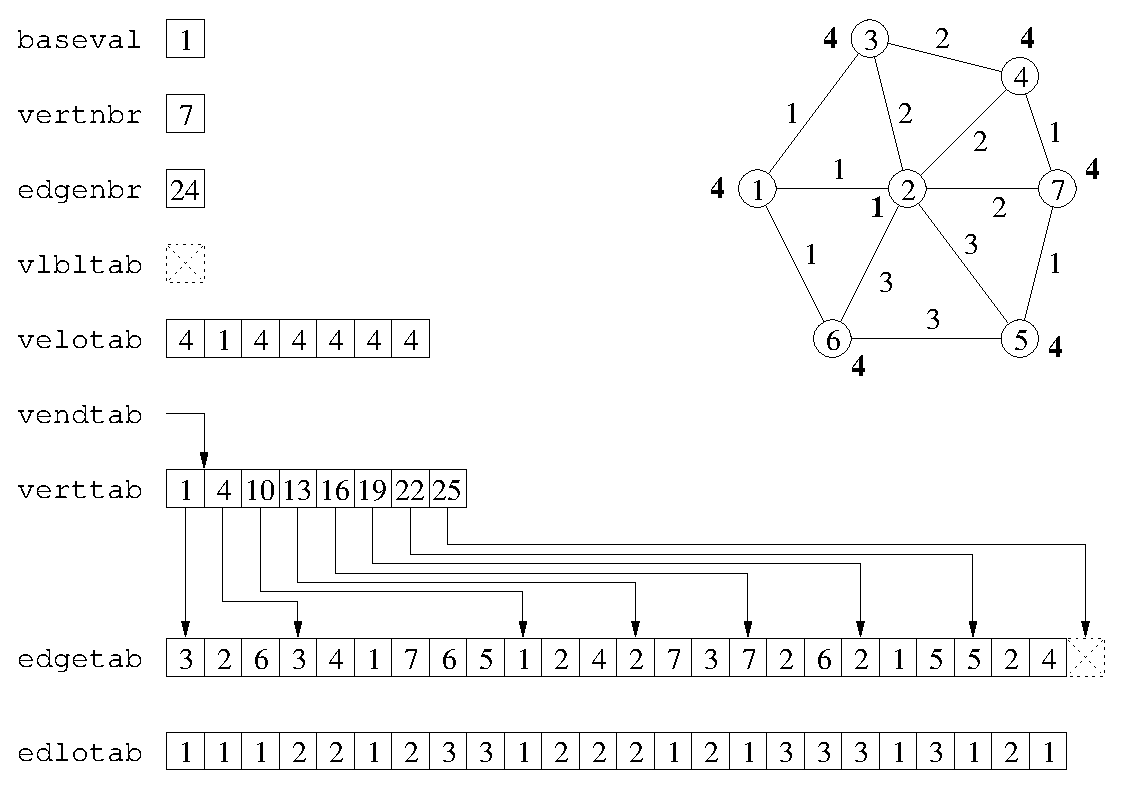
\includegraphics[scale=0.47]{s_f_gr1.eps}
\caption{Sample graph and its description using a compact edge
array. Numbers within vertices are vertex indices, bold numbers
close to vertices are vertex loads, and numbers close to edges are
edge loads. Since the edge array is compact, $\mathtt{verttax}$ is
of size $\mathtt{vertnbr} + 1$ and $\mathtt{vendtax}$ points to
$\mathtt{verttax} + 1$.}
\label{fig-lib-graf-one}
\end{figure}

\begin{figure}
\centering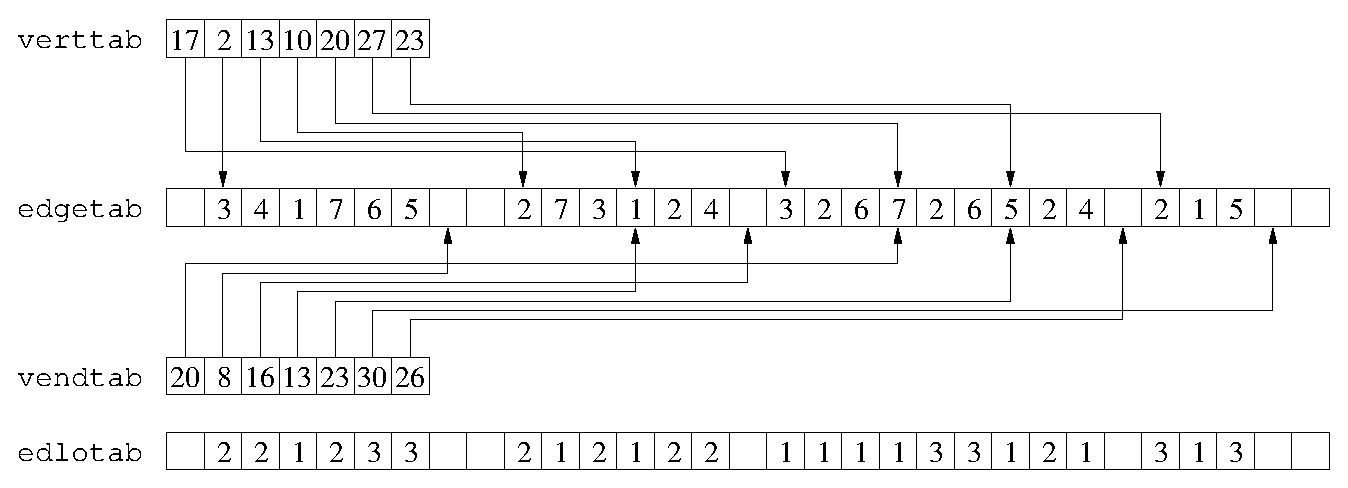
\includegraphics[scale=0.47]{s_f_gr2.eps}
\caption{Adjacency structure of the sample graph of
Figure~\protect\ref{fig-lib-graf-one} with disjoint edge and
edge load arrays. Both $\mathtt{verttax}$ and $\mathtt{vendtax}$ are
of size $\mathtt{vertnbr}$. This allows for the handling of dynamic
graphs, the structure of which can evolve with time.}
\label{fig-lib-graf-two}
\end{figure}

Dynamic graphs can be handled elegantly by using the
$\mathtt{vendtax}$ array. In order to dynamically manage graphs, one
just has to allocate $\mathtt{verttax}$, $\mathtt{vendtax}$ and
$\mathtt{edgetax}$ arrays that are large enough to contain all of the
expected new vertex and edge data. Original vertices are labeled
starting from $\mathtt{baseval}$, leaving free space at the end of the
arrays. To remove some vertex $i$, one just has to replace
$\mathtt{verttax[}i\mathtt{]}$ and
$\mathtt{vendtax[}i\mathtt{]}$ with the values of
$\mathtt{verttax[\lbt vertnbr}\lbt -1\mathtt{]}$ and
$\mathtt{vendtax[\lbt vertnbr}\lbt -1\mathtt{]}$, respectively, and
browse the adjacencies of all neighbors of former vertex
$\mathtt{vertnbr}-1$ such that all $(\mathtt{vertnbr}-1)$ indices are
turned into $i$s. Then, $\mathtt{vertnbr}$ must be decremented.

To add a new vertex, one has to fill $\mathtt{verttax[\lbt vertnbr}
-1\mathtt{]}$ and $\mathtt{vendtax[\lbt vertnbr}\lbt -1\mathtt{]}$
with the starting and end indices of the adjacency sub-array of the
new vertex. Then, the adjacencies of its neighbor vertices must also
be updated to account for it. If free space had been reserved at the
end of each of the neighbors, one just has to increment the
$\mathtt{vendtax[}i\mathtt{]}$ values of every neighbor $i$, and add
the index of the new vertex at the end of the adjacency sub-array. If
the sub-array cannot be extended, then it has to be copied elsewhere
in the edge array, and both $\mathtt{verttax[}i\mathtt{]}$ and
$\mathtt{vendtax[}i\mathtt{]}$ must be updated accordingly. With
simple housekeeping of free areas of the edge array, dynamic arrays
can be updated with as little data movement as possible.

\subsection{\texttt{Hgraph}}
\label{sec-data-hgraph}

The \texttt{Hgraph} structure holds all the information necessary to
represent and perform computations on a \textit{halo} graph. This term
refers to graphs some vertices of which are kept to preserve accurate
topological information, but are usually not subject to actual
computations. These \textit{halo vertices} are collectively referred
to as the \textit{halo} of the graph. Halo graphs are notably used in
sparse matrix reordering, where, in the process of nested dissection,
a graph is cut into three pieces: a vertex separator, and two
separated parts. Each of these parts must preserve the real degree
information attached to all their vertices, including those next to
the separator. If halo graphs were not used, the degrees of these
vertices would appear smaller than what they really are in the whole
graph. Preserving accurate degree information is essential for
algorithms such as the \textit{minimum degree} vertex ordering
method. Some vertex separation algorithms also aim at balancing halo
vertices; in this case, separators will be computed on halos, but this
information will not be preserved once a separator has been computed
on the regular vertices.

Halo graphs exhibit specific structural and topological properties,
illustrated in Figure~\ref{fig-lib-hgraf-one}. In order to distinguish
easily halo vertices from regular vertices and write efficient
algorithms, halo vertices have the highest vertex indices in the
graph. Because the degrees of halo vertices need not be preserved, no
edges connect two halo vertices; the adjacency of halo vertices is
only made of regular vertices. Also, in the adjacency arrays of
regular vertices, all non-halo vertices are placed before halo
vertices. All these properties allow one to easily induce the non-halo
graph from some halo graph, without having to create new adjacency
arrays. An additional vertex index array is present just for this
purpose.

\begin{figure}
\centering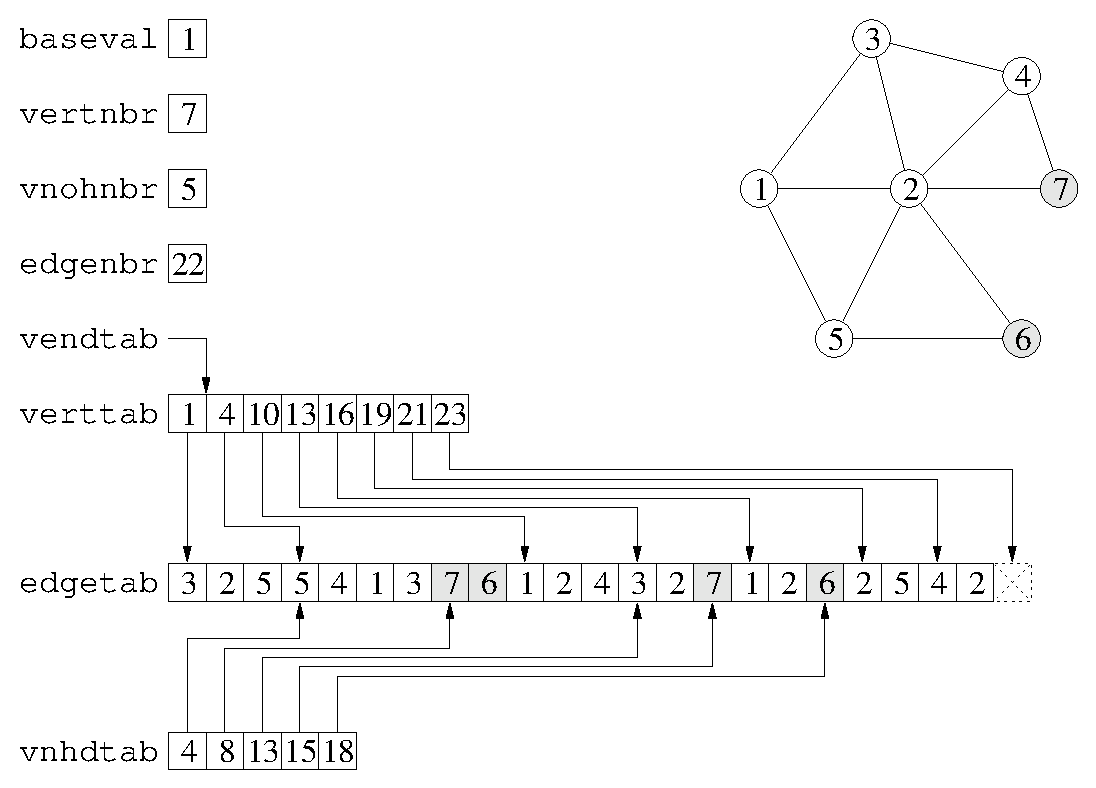
\includegraphics[scale=0.47]{m_f_gr3.eps}
\caption{Sample halo graph and its description using a compact edge
array. Numbers within vertices are vertex indices. Greyed values
are indices of halo vertices. Halo vertices have the highest indices
in the graph, and are placed last in the adjacency sub-arrays of each
non-halo vertex.}
\label{fig-lib-hgraf-one}
\end{figure}

Halo graph fields have the following meaning:
\begin{itemize}
\iteme[\texttt{s}]
Underlying source graph that contains all regular and halo
vertices. This is where to search for fields such as
$\mathtt{baseval}$, $\mathtt{vertnbr}$, $\mathtt{vertnnd}$,
$\mathtt{verttax}$, $\mathtt{vendtax}$, etc.
\iteme[\texttt{vnohnbr}]
Number of non-halo vertices in graph. Hence, $0 \leq \mathtt{vnohnbr}
\leq \mathtt{s.vertnbr}$.
\iteme[\texttt{vnhdtax}]
Array of after-last indices in $\mathtt{s.edgetax}$ of non-halo vertex
adjacency sub-arrays. Since this information only concerns non-halo
vertices, $\mathtt{vnhdtax}$ is of size $\mathtt{vnohnbr}$, not
$\mathtt{vertnbr}$.
For any non-halo vertex $i$, with $\mathtt{baseval} \leq i <
(\mathtt{vnohnbr} + \mathtt{baseval})$, the indices of the non-halo
neighbors of $i$ are stored in $\mathtt{s.edgetax}$ from $\mathtt{s.edgetax}\lbt
\mbox{\texttt{[}}\mathtt{s.verttax}\mbox{\texttt{[}}i\mbox{\texttt{]]}}$
to $\mathtt{s.edgetax}\lbt
\mbox{\texttt{[}}\mathtt{vnhdtax}\mbox{\texttt{[}}i\mbox{\texttt{]}} -
1\mbox{\texttt{]}}$, inclusive, and its halo neighbors are stored from
$\mathtt{s.edgetax}\lbt
\mbox{\texttt{[}}\mathtt{vnhdtax}\mbox{\texttt{[}}i\mbox{\texttt{]]}}$
to $\mathtt{s.edgetax}\lbt
\mbox{\texttt{[}}\mathtt{s.vendtax}\mbox{\texttt{[}}i\mbox{\texttt{]}} -
1\mbox{\texttt{]}}$, inclusive.
\iteme[\texttt{vnlosum}]
Sum of non-halo vertex loads. Hence, $0 \leq \mathtt{vnlosum}
\leq \mathtt{s.velosum}$.
\iteme[\texttt{enohnbr}]
Number of non-halo arcs in graph. Hence, $0 \leq \mathtt{enohnbr}
\leq \mathtt{s.edgenbr}$.
\end{itemize}

\subsection{\texttt{Kgraph}}
\label{sec-data-kgraph}

The \texttt{Kgraph} structure holds all the information necessary to
compute a k-way (re)mapping of some graph onto a target architecture.
Consequently, it contains a \texttt{Graph}, defined as field
\texttt{s}, and a reference to an \texttt{Arch}, through the field
\texttt{m.archptr}, as well as two \texttt{Mapping} structures: one
for the current mapping to compute, and one to store the old mapping
from which to remap. Additional information comprise data to model the
cost of remapping, and data associated with the state and cost of the
current mapping: list of frontier vertices, load of each partition
domain, plus the execution context for multi-threading execution.

The \texttt{Graph} structure is internal to the \texttt{Kgraph}
because every new \texttt{Kgraph} contains a different graph topology
(\eg, a band graph or a coarsened graph). The \texttt{Arch} is
accessed by reference because it is constant data which can be shared
by many \texttt{Kgraph}s. For the sake of consistency, the
\texttt{grafptr} fields of each mapping \texttt{m} and \texttt{r.m}
must point to \texttt{\&s}, while their two \texttt{archptr} fields
must point to the same target architecture. This redundency is the
price to pay for lighter memory management.

\subsubsection{Mappings}

The \texttt{domnorg} field, which must contain a valid domain in the
architecture \texttt{m.archptr}, is the starting point for the k-way
mapping. This domain may be smaller than the full architecture when
parallel partitioning is performed: in this case, each process may
receive a separate subgraph and sub-architecture to work on.

Each of the two mappings has its own specificities. The current
mapping, defined as field \texttt{m}, is never incomplete: all the
cells of its \texttt{m.parttax} array are non-negative values that index
a valid domain in the domain array \texttt{m.domntab}. These domains
are all subdomains of the architecture referenced through field
\texttt{m.archptr}. More restrictively, the domains attached to
non-fixed vertices must be included in \texttt{domnorg}, which may be
smaller.

The current mapping evolves with time, according to the various
algorithms that the user can activate in the strategy string. These
algorithms will create derived \texttt{Kgraph}s (\eg, band graphs or
coarsened graphs), to which mapping methods will be applied, before
the result is ported back to their parent \texttt{Kgraph}. Depending
on the kind of the derived graph, the \texttt{m.parttax} array may be
specific, but the \texttt{m.domntab} array will always be ported back
as is. Consequently, in order to save memory copying, the policy which
is implemented is that the derived \texttt{Kgraph} gets the pointer to
the \texttt{m.domntab} of its parent, while the latter is set to
\texttt{NULL}. The derived graph can therefore reallocate the array
whenever needed, without the risk of an old, invalid, pointer being
kept elsewhere. Then, when the processing of the derived
\texttt{Kgraph} ends, the most recent pointer is copied back to the
\texttt{m.domntab} field of the parent graph, and the
\texttt{m.parttax} array is updated accordingly, after which the
derived \texttt{Kgraph} can be destroyed without freeing the
pointer.

The old mapping, defined as field \texttt{r.m},
may contain incomplete mapping information: some of the cells of its
\texttt{r.m.parttax} array may be equal to \texttt{-1}, to indicate
that no prior mapping information is available (\eg, when the vertex
did not exist in the previous mapping). Since old mappings do not
change, the \texttt{r.m.domntab} field can be shared among all derived
\texttt{Kgraph}s. It is protected from double memory freeing by not
setting the \texttt{MAPPING\lbt FREE\lbt DOMN} flag in field
\texttt{r.m.flagval}.

\subsection{\texttt{Mapping}}
\label{sec-data-mapping}

The \texttt{Mapping} structure defines how individual vertices of a
\texttt{Graph} are mapped individually onto (parts of) an
\texttt{Arch}. A mapping is said \textit{complete} if all source graph
vertices are assigned to terminal target domains, \ie, individual
vertices of the target architecture, or \textit{partial} if at least
one of the source graph vertices is assigned to a target domain that
comprises more than one vertex. In the course of the graph mapping
process, the destination of source vertices are progressively refined,
from an initial target domain that usually describes the whole of the
target architecture, to terminal domains.

Since \texttt{ArchDom}, the data structure that describes target
architecture domains, is big and costly to handle (\eg, to compare if
two \texttt{ArchDom}s are identical), the handling of domains in
mapping is indirect: in the part array \texttt{parttax}, each vertex
is assigned an integer domain index that refers to a domain located in
the domain array \texttt{domntab}. Hence, when two graph vertices have
the same index in \texttt{parttax}, they belong to the same domain and
induce no communication cost. However, the opposite is false: two
vertices may have a different index in \texttt{parttax} and yet belong
to the same target domain. This is for instance the case when one of
the vertices is a fixed vertex that has been set to a specific
terminal domain at initialization time, and one of its neighbors is
successively mapped to smaller and smaller subdomains that eventually
amount to the same terminal domain.

In the case of a remapping, the mapping information regarding the
former placement of the vertices may be incomplete, \eg, because the
vertex did not exist before. Such a mapping is said to be
\textit{incomplete}. It is characterized by the fact that some cells
of the \texttt{parttax} array are equal to \texttt{-1}, to indicate an
unknown terminal domain number. To allow for this, the mapping must
have the \texttt{MAPPING\lbt INCOMPLETE} flag set. Incomplete mappings
are only valid when holding remapping information; new mappings being
computed must have all their \texttt{parttax} cells set with
non-negative values that point to valid domains in the
\texttt{domntab} array. New mappings can therefore only be partial or
complete.

When a mapping is initialized, all \texttt{parttax} values for
non-fixed vertices are set to index~$0$, and \texttt{domntab[0]} is
set to the root domain for the mapping. In the general case for
centralized mapping, the initial domain is equal to
\texttt{archDomFrst(archptr)}. However, when a centralized mapping
process is launched as a part of a distributed mapping process, the
initial domain may be a subset of the whole target architecture.

There is no obligation for the \texttt{domntab} array to contain only
one instance of some target domain. On the contrary, as described
above, the same domain may appear at least twice: once for fixed
vertices, and once for non-fixed vertices on which mapping algorithms
are applied. However, for efficiency reasons (\eg, avoiding to compute
vertex distances that are equal to zero), it is preferable that
duplicate domains are avoided in the \texttt{domntab} array. This is
the case by nature with recursive bipartitioning, as the domains
associated with branches of the biparitioning tree are all distinct.

Making the distinction between fixed and non-fixed vertices, which is
relevant to mapping algorithms, is not in the scope of the
\texttt{Mapping} data structure, which only represents a global
state. This is why no data related to fixed vertices is explicitly
present in the mapping itself (it may be found, \eg, in the
\texttt{Kgraph} data structure).
However, for handling fixed vertices in an efficient way, the
semantics of the \texttt{Mapping} data structure is that all domains
that are associated with fixed vertices must be placed first in the
\texttt{domntab} array. The purpose of this separation is because,
when the imbalance of a mapping is computed, the loads of non-fixed
vertices that belong to some (partial) domain and of fixed vertices
that belong to domains that are subdomains of this domain have to be
aggregated. This aggregation procedure is made easier if both types of
domains are kept separate. For efficiency reasons, fixed domains
should appear only once in the fixed part of \texttt{domntab}.
\\

The \texttt{Mapping} structure is mainly used within the
\texttt{Kgraph} structure, which contains two instances of it: one for
the current mapping to be computed, and one for the old mapping, in
the case of remapping. The building of a \texttt{Kgraph} from another
one (\eg, when creating a band graph or a coarsened graph) may lead to
situations in which some \texttt{Mapping} arrays may be re-used, and
thus should not be freed when the derived \texttt{Mapping} is
freed. This is why the \texttt{Mapping} structure contains flags to
record whether its arrays should be freed or not. These flags are the
following:
\begin{itemize}
\iteme[\texttt{MAPPINGFREEDOMN}]
  Set if the domain array has to be freed when the mapping is freed. A
  common case for sharing the domain array is when a coarser
  \texttt{Kgraph} is computed: the domain array of the coarse old
  mapping can re-use that of the fine old mapping.
\iteme[\texttt{MAPPINGFREEPART}]
  Set if the part array has to be freed when the mapping is freed. A
  common case for sharing the part array is when the user part array
  is kept as the part array for the initial \texttt{Kgraph} current
  mapping structure.
\end{itemize}

The main fields of the \texttt{Mapping} data structure are the following:
\begin{itemize}
\iteme[\texttt{flagval}]
  Set of flags indicating whether the \texttt{parttax} and
  \texttt{domntab} have to be freed on exit.
\iteme[\texttt{grafptr}]
  Pointer to the \texttt{Graph} associated with the mapping, that
  gives access to the base value \texttt{grafptr->\lbt baseval} and
  the number of source vertices \texttt{grafptr->\lbt vertnbr}.
\iteme[\texttt{archptr}]
  Pointer to the \texttt{Arch} associated with the mapping, that is
  necessary to perform all distance computations on the mapping.
\iteme[\texttt{parttax}]
  Based array of \texttt{Anum}s, of size \texttt{grafptr->\lbt
  vertnbr}, that provides the index of the target domains onto which
  all graph vertices are currently mapped. Indices are un-based.
\iteme[\texttt{domntab}]
  Un-based array of \texttt{ArchDom}s, of size \texttt{domnmax}, that
  stores the target domains to which source graph vertices are
  indirectly associated through the \texttt{parttax} array.
\iteme[\texttt{domnnbr}]
  Number of target domain slots currently used in
  \texttt{domntab}. After a mapping is initialized, $1 \leq
  \mbox{\texttt{domnnbr}} < \mbox{\texttt{domnmax}}$, because source
  graph vertices must be associated to some domain, hence
  \texttt{domntab} should at least contain one domain.
\iteme[\texttt{domnnbr}]
  Number of target domain slots currently used in
  \texttt{domntab}.
\iteme[\texttt{domnmax}]
  Size of the \texttt{domntab} array.
\iteme[\texttt{mutedat}]
  When multi-threading is activated, allows to create critical
  sections to update the mapping data in a thread-safe manner.
\end{itemize}
